\documentclass[]{article}
\usepackage{lmodern}
\usepackage{amssymb,amsmath}
\usepackage{ifxetex,ifluatex}
\usepackage{fixltx2e} % provides \textsubscript
\ifnum 0\ifxetex 1\fi\ifluatex 1\fi=0 % if pdftex
  \usepackage[T1]{fontenc}
  \usepackage[utf8]{inputenc}
\else % if luatex or xelatex
  \ifxetex
    \usepackage{mathspec}
  \else
    \usepackage{fontspec}
  \fi
  \defaultfontfeatures{Ligatures=TeX,Scale=MatchLowercase}
\fi
% use upquote if available, for straight quotes in verbatim environments
\IfFileExists{upquote.sty}{\usepackage{upquote}}{}
% use microtype if available
\IfFileExists{microtype.sty}{%
\usepackage{microtype}
\UseMicrotypeSet[protrusion]{basicmath} % disable protrusion for tt fonts
}{}
\usepackage[unicode=true]{hyperref}
\hypersetup{
            pdfborder={0 0 0},
            breaklinks=true}
\urlstyle{same}  % don't use monospace font for urls
\usepackage{graphicx,grffile}
\makeatletter
\def\maxwidth{\ifdim\Gin@nat@width>\linewidth\linewidth\else\Gin@nat@width\fi}
\def\maxheight{\ifdim\Gin@nat@height>\textheight\textheight\else\Gin@nat@height\fi}
\makeatother
% Scale images if necessary, so that they will not overflow the page
% margins by default, and it is still possible to overwrite the defaults
% using explicit options in \includegraphics[width, height, ...]{}
\setkeys{Gin}{width=\maxwidth,height=\maxheight,keepaspectratio}
\IfFileExists{parskip.sty}{%
\usepackage{parskip}
}{% else
\setlength{\parindent}{0pt}
\setlength{\parskip}{6pt plus 2pt minus 1pt}
}
\setlength{\emergencystretch}{3em}  % prevent overfull lines
\providecommand{\tightlist}{%
  \setlength{\itemsep}{0pt}\setlength{\parskip}{0pt}}
\setcounter{secnumdepth}{0}
% Redefines (sub)paragraphs to behave more like sections
\ifx\paragraph\undefined\else
\let\oldparagraph\paragraph
\renewcommand{\paragraph}[1]{\oldparagraph{#1}\mbox{}}
\fi
\ifx\subparagraph\undefined\else
\let\oldsubparagraph\subparagraph
\renewcommand{\subparagraph}[1]{\oldsubparagraph{#1}\mbox{}}
\fi

% set default figure placement to htbp
\makeatletter
\def\fps@figure{htbp}
\makeatother


\date{}

\begin{document}

Igiene 21/11/2016

Dott.ssa A.Odone

Sbobinatore: Nicolò Gallina

Argomenti: Determinanti di salute, One Health, Health in all polices,
dettaglio dei singoli determinanti di salute

\textbf{News del giorno} (sottosezione)

News del giorno, presa dal bollettino della società italiana di igiene,
si parla di introdurre la scuola di specialità in medicina generale (che
adesso è a carico delle singole regioni) incardinata nel circuito
universitario. L'idea è quella di incaricare l'ambito dei servizi
l'organizzazione dei nuovi percorsi di studio per i medici di medicina
generale. Perché i medicini di medicina generale hanno un'importante
ruolo nella comunicazione sanitaria e nella prevenzione.

\textbf{Determinanti di salute} (sezione)

Per determinanti intendiamo un fattore, ovvero ciò che determina. I
determinanti della salute sono quindi quei fattori che impattano sullo
stato di salute.

Alcuni esempi possono essere:

\begin{itemize}
\item
  Dieta
\item
  Età
\item
  Sesso, genere
\item
  Attività fisica
\item
  Fumo
\item
  Consumo di alcol
\item
  Predisposizioni genetiche
\item
  Ambiente lavorativo
\item
  Condizioni socio-economiche
\item
  Inquinamento
\item
  istruzione
\end{itemize}

Per determinanti di salute si intendono i molti e interconnessi fattori
che determinano la salute degli individui e delle comunità, includono
tre grossi capitoli:

1)Contesto economico sociale in cui le persone vivono;

2)L'ambiente fisico;

3)Le caratteristiche individuali delle persone e i comportamenti.
(definizione dell'OMS).

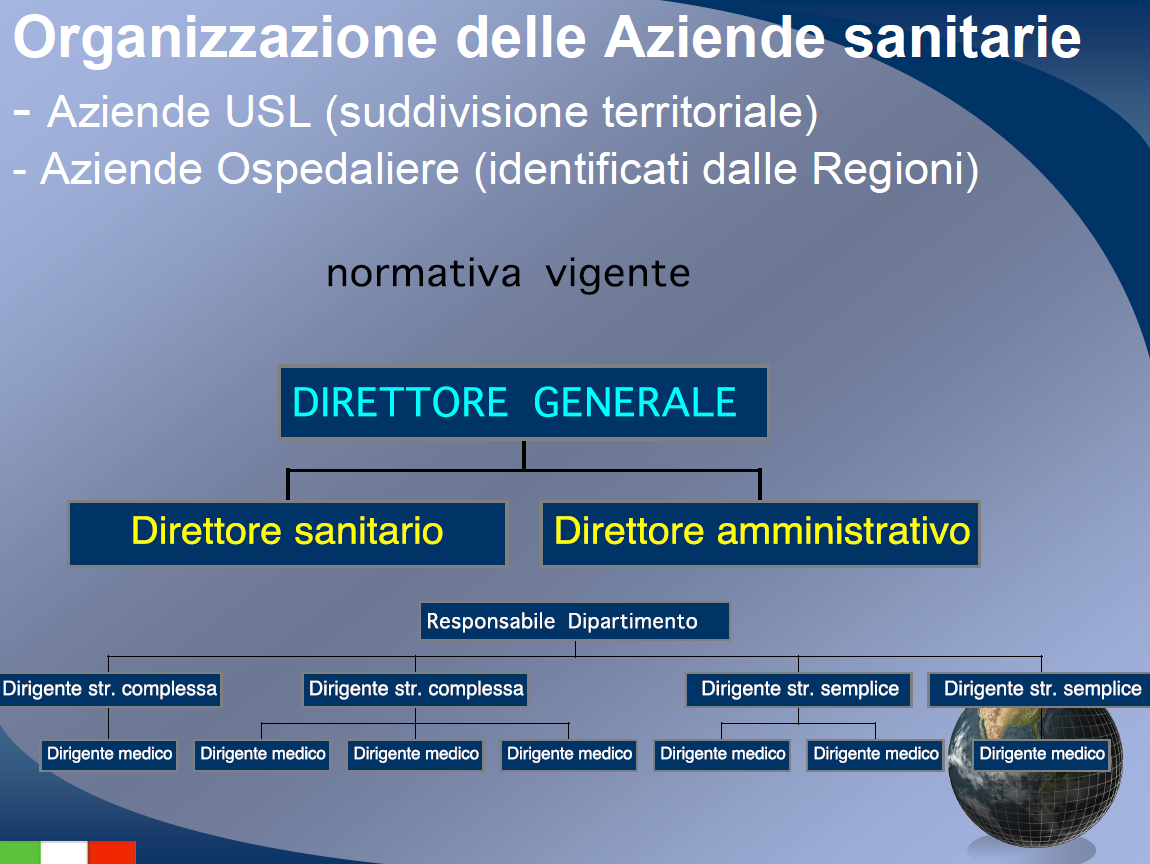
\includegraphics[width=6.68889in,height=5.02639in]{media/image1.png}

Il Grafico vi presenta la distribuzione dei determinanti nelle
popolazioni in base al peso che hanno. Alcuni determinanti di salute
sono modificabili altri invece immodificabili. Le predisposizioni
genetiche sono ad es dei determinanti di salute immodificabili e quindi
non adressabili da interventi di prevenzione primaria. Altri
determinanti sono le caratteristiche sociali e della società, i
comportamenti e l'accesso alla cure mediche. Il grafico non vuole essere
esaustivo quanto far vedere l'importanza dei diversi determinanti di
salute dove la componente familiare genetica non è che una percentuale
minima. Questo significa che si può fare molto per modificare la salute
del singolo o di una popolazione con un approccio di sanità pubblica
andando ad adressare quelli che sono i determinanti modificabili, ovvero
quelli associati all'ambiente e al comportamento.

I modelli che sono stati proposti in letteratura per classificare i
determinanti di salute o di malattia sono pochi; Quello più famoso e
utilizzato e presente in questa immagine, è un modello sviluppato nel
'91 da due ricercatori dell'Università di Liverpool. I determinanti di
salute sono distribuiti attorno agli individui e alle persone, persone
che hanno particolari caratteristiche genetiche (voi avete detto il
sesso per esempio) attorno a cui con livelli di prossimità decrescente
sono distribuiti gli altri determinanti di salute. Come detto l'OMS
distingue in 3 grandi capitoli, i fattori di rischio individuali legati
allo stile di vita che sono quelli più prossimali ai singoli individui
(dieta, fumo, consumo di alcol, stili di vita e comportamenti) su cui si
collocano le caratteristiche delle comunità su cui si collocano con una
collocazione ancor più distale le caratteristiche ecologiche (l'ambiente
fisico, ambiente culturale, le indicazioni socio economiche)

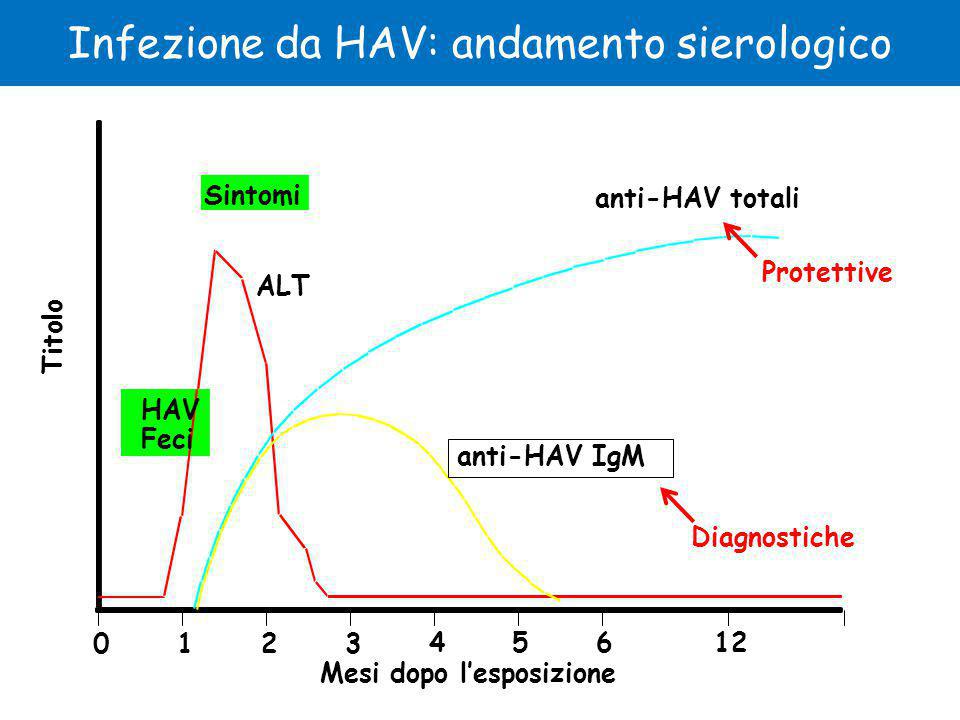
\includegraphics[width=6.68889in,height=5.01319in]{media/image2.png}

Se voi prendete questo come riferimento riuscite a capire quest'altro
grafico.

Partiamo dai determinanti più distali che sono: il contesto
socio-economico e politico, in che modo il contesto socio economico e
politico può influenzare sulla salute del singolo individuo? Per esempio
\textbf{l'istruzione} (education) può influenzare lo stato di salute?
Voi pensate ci sia una correlazione educazione del soggetto e outcome di
malattia? C'è una correlazione positiva o negativa tra grado di
scolarità e per esempio la mortalità? La risposta è si, i dati di
letteratura dimostrano che c'è una associazione le persone con una
scolarità più alta hanno una miglior salute. Quello che è interessante
capire è come mai succede ciò? Cioè quali sono i diversi e interconnessi
meccanismi che mediano questa associazione. Per esempio uno è associato
all'educazione sanitaria, è dimostrato che persone che hanno una
scolarità minore sono meno informate rispetto ai rischi di salute e
quindi attuano comportamenti più a rischio con il risultato di uno stato
di salute peggiore. Altri meccanismi possono essere comportamenti,
abitudini e stili di vita ``peggiori'' come una alimentazione più
economica che è meno varia e quindi influisce sull'outcome di salute che
sarà peggiore. Altro esempio è \textbf{l'attività lavorativa}
(occupation) è un determinante di salute, in che modo l'attività
lavorativa influenza la salute delle persone? Esempio il numero di ore
di lavoro, un datore di lavoro estremamente oppressivo, mansioni più
manuali sono legati ad outcome di malattia correlate all'usura fisica
maggiore oppure l'esposizione in ambito lavorativo, l'ambiente di lavoro
che può causare infortuni.

Una cosa da non dimenticare è l'accesso alle cure, a parità di stato
economico, di educazione e di occupazione lavorativa quello che media un
buono stato di salute è l'accesso ai servizi sanitari sia come offerta
dei sistemi sanitari (che possono essere più o meno ricchi) sia della
domanda (cioè del cittadino che ha i mezzi sia materiali che
intellettuali di accedere alle cure messe a disposizione dal SSN).

\textbf{ONE HEALTH (UNA SALUTE)} (Paragrafo)

Il concetto di one health riconosce che la salute degli esseri umani è
legata alla salute degli animali e dell'ambiente.

In che modo la salute animale può influenzare la salute umana? Esempio
le zoonosi sono l'esempio classico di associazione tra salute umana e
animale; le antibiotico resistenze sono un altro esempio perché gli
antibiotici vengono usati anche per loro.

One health promuove l'applicazione di un approccio collaborativo,
multidisciplinare, intersettoriale e coordinato per affrontare quelli
che sono i rischi potenziali o già esistenti che hanno origine
dall'interfaccia tra ambiente e animali ed ecosistemi umani.

C'è quindi il concetto di salute unica come fosse un ``ombrello'' che
ricopre la salute ambientale, l'ecologia, la medicina veterinaria la
sanità pubblica la medicina clinica umana, la microbiologia in maniera
interconnessa.

\textbf{HEALTH IN ALL POLICES (Salute in tutte le politiche)}
(paragrafo)

Tutte le politiche economiche, agricole, ambientali, di educazioni,
praticamente tutti i ministeri dovrebbero tener conto delle potenziali
implicazioni sulla salute che le loro decisioni hanno.

Per essere efficace la politica sanitaria deve coinvolgere anche le
altre politiche.

Il concetto di ``Città sana'' è un luogo ideale in cui vivere, poco
inquinata, pulita, con bassa criminalità. Bassa criminalità può voler
dire bassa prevalenza di infortuni a scippi violenti, pestaggi,
benessere psicologico nel vivere in una città sicura.

Se voi pensate ad un determinante dovete poi riflettere su quali siano i
meccanismi con cui questo determinante impatta sulla salute e quindi su
cui noi possiamo lavorare.

Le fonti di inquinamento in una città sono riscaldamento, traffico,
rifiuti, inquinamento acustico, acque reflue e quindi avendo capito i
fattori, le politiche di infrastructure, planning and trasport che vanno
verso la direzione di una città sana possono essere: Piste ciclabili
perché riducono il traffico, si abbassa l'inquinamento e migliora la
salute. Si può favorire l'uso dei mezzi pubblici con sconti sui
trasporti, bike sharing, le ZTL.

\textbf{Dettaglio dei determinanti di salute} (Sottosezione)

Ora analizziamo più nel dettaglio i determinanti di salute

\textbf{Dieta} (Paragrafo)

Può essere sia un determinante di salute che di malattia. L'indice di
massa corporea BMI è un indice che si utilizza per valutare l'obesità.
Ci sono molti dati disponibili su quella che è la distribuzione del
sovrappeso e dell'obesità in diverse fasce d'età. L'Italia per la
distribuzione di una serie di determinanti di salute quali la dieta, gli
aspetti culturali e l'attività fisica si colloca in una posizione
virtuosa rispetto ad altri paesi europei per quanto riguarda la
distribuzione di sovrappeso e obesità nell'età adulta. Si crede sia
legato ad abitudini alimentari genericamente più salutari rispetto a
paesi nordici, quello che è preoccupante e che emerge dai dati è invece
l'obesità e il sovrappeso nella popolazione infantile. L'obesità
infantile in Italia è maggiore rispetto ad altri paesi; voi come
interpretereste questo dato? Cioè differenza di obesità tra adulto e
bambino? Non c'è una risposta, ma si può interpretare questo dato
dicendo che è un dato negativo perché c'è più probabilità che un bambino
in sovrappeso diventi un adulto in sovrappeso. Perché adesso gli adulti
sono normopeso rispetto ai colleghi europei mentre le popolazioni
infantili non lo sono? Quali potrebbe essere la distribuzione di
determinanti che influisce su questo pattern? Per esempio nel tempo si è
modificata la sedentarietà e l'abitudine negli stili di vita e questo
potrebbe essere la ragione di questa discrepanza, altri motivi la dieta
può sembrare che i benefici della dieta mediterranea si stiano perdendo.
Se notiamo la distribuzione regionale, le regioni del sud hanno una
prevalenza sulla distribuzione di sovrappeso e obesità rispetto alle
regioni del nord. Questo si riferisce alla dieta, agli stili di vita.

In Italia a livello di comunicazione sono a disposizione degli strumenti
per rendere i cittadini ``empowerd'' istruiti e colti per quanto
riguarda le abitudini alimentari e gli stili di vita. Il progetto Cuore,
sviluppato dall'istituto superiore di sanità, ne è un esempio, in cui i
cittadini immettendo su una schermata video alcune caratteristiche tipo
il sesso, età, pressione e abitudine al fumo, potevano avere una stima
della loro probabilità ad andare incontro ad un evento cardiovascolare.
E' un esempio di quello che si può fare per promuovere a diversi livelli
stili di vita corretti.

\textbf{Attività Fisica} (Paragrafo)

Tutti sanno che l'attività fisica ha un impatto positivo su diversi
outcome di salute. Quello che è certo è che l'inattività fisica è un
fenomeno in aumento, perché secondo voi? Un esempio può essere che le
attuali attività ricreative dei bambini vertono più su videogiochi, Ipad
piuttosto che attività movimentate all'aperto. Altri fattori che portano
ad una riduzione dell'attività fisica nella nostra società possono
essere lavoro, come uno va al lavoro, studio.

L'inattività fisica è al quarto posto come causa di morte dovute a
malattie croniche quali disturbi cardiaci, ictus, diabete, patologie
neoplastiche contribuendo ad oltre 3 milioni di morti evitabili a
livello mondiale ogni anno. Gli aumenti dei livelli di obesità infantile
e adulta è strettamente correlato all'inattività fisica.

Il sistema PASSI è un sistema di monitoraggio degli stili di vita e dei
comportamenti in prevenzione in Italia che si basa su questionari
somministrati ad un campione rappresentativo della popolazione italiana.
Questi dati si basano su dati self riportati, per esempio il sistema
calcola l'obesità non andandola a misurare direttamente su ogni
individuo, ma chiedendo ai singoli individui intervistati di auto
dichiarare il proprio peso. Quanto secondo voi il dato self riportato
del peso o dell'altezza si discosta dalla realtà? Generalmente il peso è
sottostimato e l'altezza e sovrastimata, questo porta ad un BMI
matematicamente sottostimato.

Benché al sud l'alimentazione sia più sana sia per disponibilità di
prodotti che per andamento culturale, in realtà sovrappeso e obesità
sono maggiori legati agli aspetti quantitativi del cibo ma soprattutto
alla distribuzione della sedentarietà rispetto alle regioni del nord.

Quello che è possibile fare con i dati PASSI è fare anche delle
inferenze vedendo anche la distribuzione in questo caso della
sedentarietà per caratteristiche socio-demografiche quali ad esempio
età, sesso, grado di istruzione e facoltà economiche.

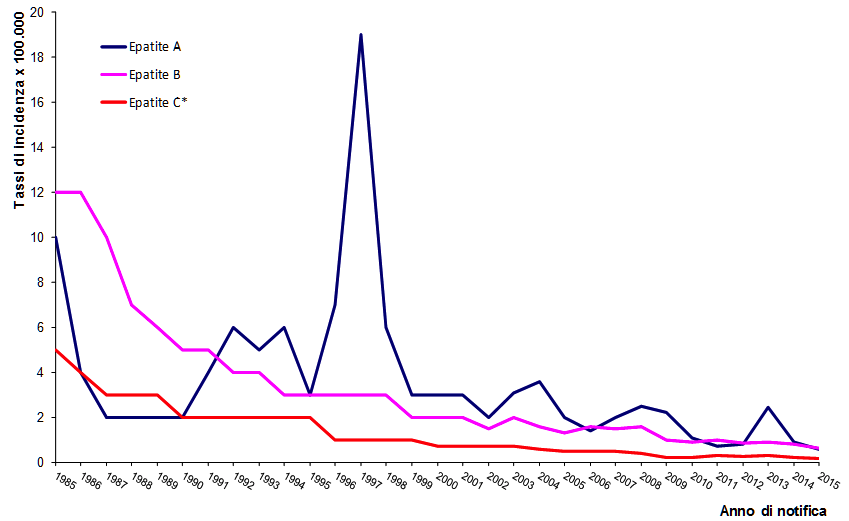
\includegraphics[width=6.68889in,height=4.98889in]{media/image3.png}

Viene descritto a parole un grafico proiettato a lezione ``Sull'asse
delle ascisse è indicato la quantità di persone, sulle ordinate vediamo
che l'età più aumenta più abbiamo una quantità maggiore di sedentari;
per quanto riguarda il sesso il sesso femminile ha una prevalenza di
sedentarietà rispetto a quello maschile; per quanto riguarda
l'istruzione è inversamente proporzionale cioè meno le persone sono
istruite e più saranno sedentarie; per quanto riguarda le difficoltà
economiche è direttamente proporzionale ovvero più avremo difficoltà
economiche e più le persone saranno sedentarie.''

Quindi in generale uno stato socio-economico inferiore, che si può
misurare attraverso il grado di istruzione, sia legato a distribuzione
maggiore del fattore di rischio sedentarietà.

\textbf{Fumo} (paragrafo)

Il 12\% dei giovani a 15 anni secondo voi fuma? Si questo è un dato non
aggiornatissimo ma corretto. Vuol dire che 12 adolescenti su 100 a 15
anni fumano.

Tabagismo (dati OMS): l'abitudine al fumo è il principale fattore di
rischio oncogeno per l'uomo. In Italia si stima che siano attribuibili
al fumo di tabacco dalle 70 alle 83mila morti all'anno. Non solo per il
rischio oncogeno in quanto al tabacco è riconosciuta causa nota o
probabile di almeno 25 patologie. Negli uomini il fumo è responsabile di
almeno il 90\% di tutte le morti per cancro al polmone e nelle donne il
55\% dei casi per un totale di circa 30mila morti all'anno in Italia. Le
azioni di contrasto al tabagismo sono finalizzate a impedire o limitare
l'inizio del fumo ed è un concetto più complicato rispetto che far
smettere di fumare. Chi si occupa di ``Tabacco control'' sa che le
azioni di contrasto possono avere come obbiettivo finale:

\begin{itemize}
\item
  impedire l'inizio del fumo
\item
  ritardarlo
\item
  favorire la disassuefazione
\item
  eliminare o ridurre l'esposizione al fumo passivo.
\end{itemize}

Prendete gli USA, io vi posso dire un grande successo della sanità
pubblica degli stati uniti e un grande insuccesso: il grande insuccesso
è l'obesità/sovrappeso/alimentazione; mentre il grande successo è la
campagna contro il fumo. Negli USA se qualcuno fuma per strada, anche
nei luoghi dove è concesso, viene guardato proprio male a dimostrazione
di come la società sia riuscita a far passare il concetto che fumare non
è per niente cool.

Secondo voi quali possono essere state le azioni intraprese dal governo
che hanno favorito questo successo? Tramite educazione, formazione,
comunicazione, le tasse sui tabacchi, gli aspetti normativi e il
consentire o meno il fumo nei luoghi chiusi pubblici.

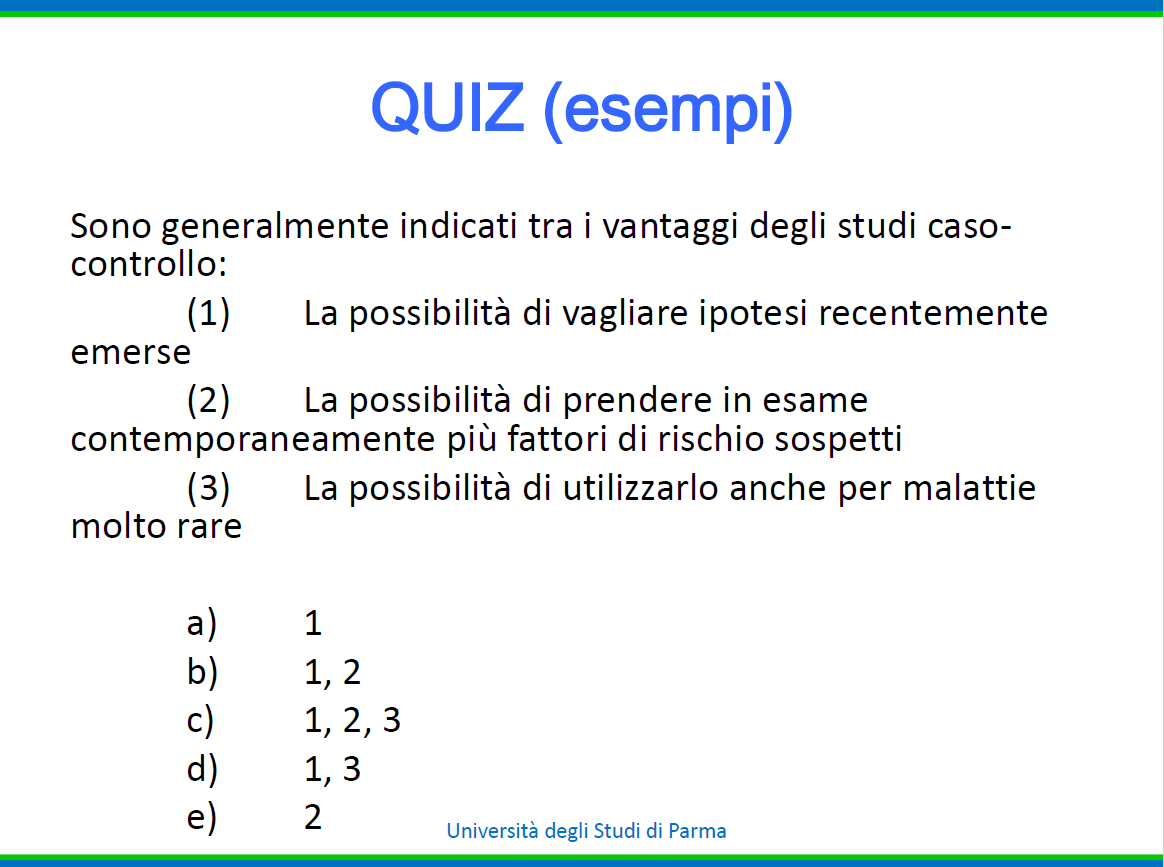
\includegraphics[width=6.68889in,height=4.98194in]{media/image4.png}

Nella slide potete vedere la distribuzione nei due sessi dell'abitudine
al fumo {[}prevalenza di fumatori per sesso dal 1993 al 2010{]} cosa
vedete? Innanzitutto possiamo dire che l'abitudine al fumo in Italia,
tutt'oggi, è ancora più prevalente nel sesso maschile e questo era
valido negli anni 90 ed è ancora valido; dalla slide possiamo ricavare
anche una seconda informazione ossia che il gap si sta riducendo nel
senso che la popolazione maschile sta riducendo l'abitudine al fumo
mentre nel sesso femminile si è assistito ad un tenue aumento di questa
prevalenza, è soprattutto la riduzione dell'abitudine fumatoria nei
maschi che ha permesso di ridurre questo gap.

\textbf{Alcol} (Paragrafo)

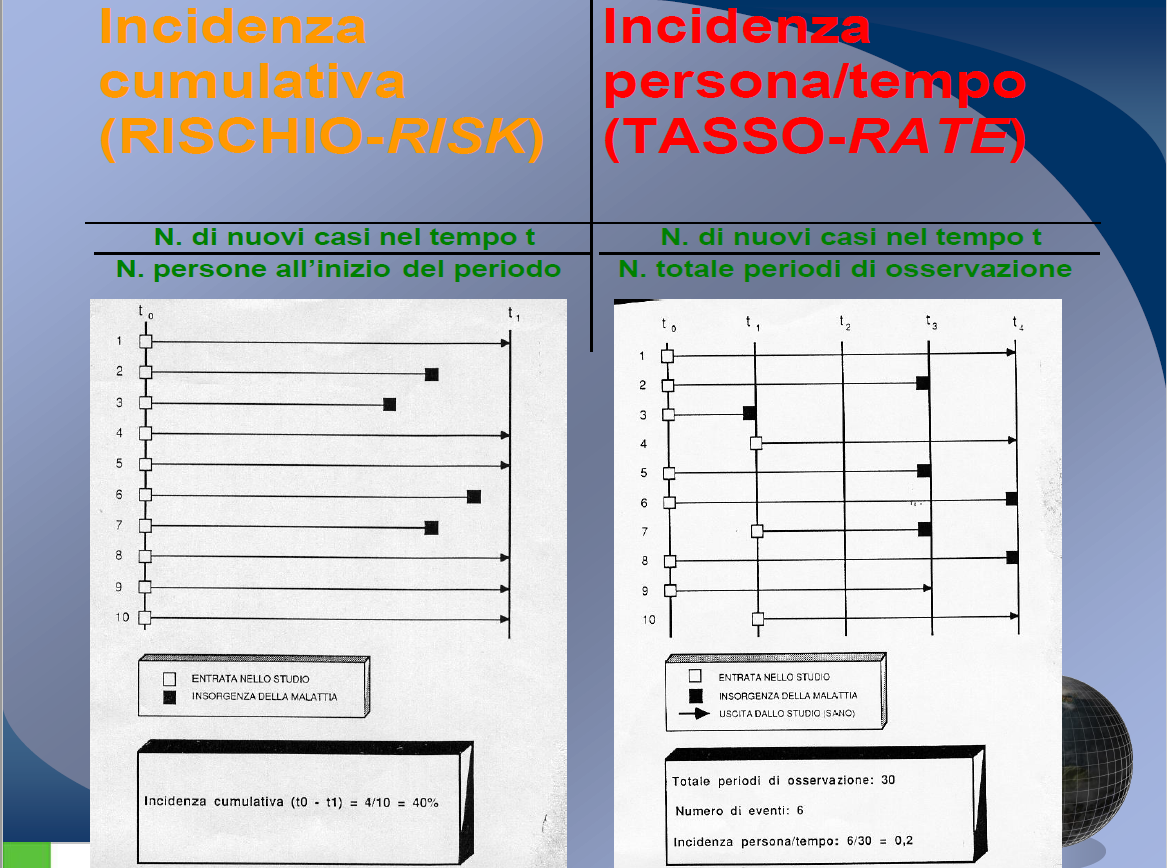
\includegraphics[width=6.68889in,height=5.00625in]{media/image5.png}

Questa tabella, presa dal vostro libro, riassume le principali patologie
attribuibili al consumo cronico di alcolici come cirrosi, epatite,
steatosi, gastrite alcolica. Anche per il consumo di alcol sia in
termini qualitativi (che tipo di alcol) che in termini quantitativi sono
interessanti le indagini condotte a livello europeo che tratteggiano
l'abitudine al consumo di alcol nei diversi stati europei. Questi sono
dei dai della FAO (sede a Roma) e sono dei dati globali nella
popolazione di età superiore ai 15 anni, valuta il consumo totale di
birra, super alcolici e vino.

Quali sono secondo voi i pattern di distribuzione del diverso consumo di
alcol negli stati europei? Il nord Europa birra, all'est super alcolici.
Quello che possiamo dire riferito ad aspetti culturali e che nel nord
del mondo c'è un approccio comportamentale al consumo di alcol rispetto
al sud dell'Europa in cui il consumo è più concentrato in alcuni giorni
della settimana (weekend), più legato ad un consumo del tipo compulsivo
legato a certe manifestazioni sociali e che questo fenomeno è un
problema di sanità pubblica, non tanto in Italia quanto in stati come
quelli scandinavi legati a possibili rischi per la salute come:
malformazioni fetali, incidenti stradali, infortuni, coma etilico,
comportamenti violenti, gravidanze non volute.

Importante è anche l'interazione fumo alcol, su cui si può sia fare un
ragionamento di tipo biologico qual è l'effetto cumulativo del consumo
di alcol e fumo sulle diverse patologie, legato però anche a quelli che
sono pattern comportamentali comuni legati alle dipendenze a determinati
stili di vita. Possiamo fare un discorso su quelli che sono gli
interventi di prevenzione primaria sull'alcol come:

\begin{itemize}
\item
  regolamentazione pubblica della pubblicità del contenuto alcolico
  delle bevande
\item
  azione di controllo della qualità dei prodotti alcoli
\item
  campagne di prevenzione sanitaria anche mirate a controllare i consumi
  alcolici nelle donne in gravidanza
\item
  iniziative per la dissuefazione
\item
  favorire il rispetto dei limiti alcolici durante la guida
\item
  regolamentazione della vendita
\item
  misure fiscali sulla vendita
\end{itemize}

Il ruolo della sanità pubblica a livello di comunicazione si deve
occupare di certi stati anche di queste problematiche che sono
considerate problematiche si sanità pubblica legate alla distribuzione
differenziale dei vari determinanti di salute (es Inghilterra dove il
tasso di gravidanze non volute è più alto della media europea).

\end{document}
